

In terms of when the order matching takes place, 
Double auction markets are generally divided into sealed-bid double 
auctions and continuous double auctions (CDA). In sealed-bid double 
auctions the orders are submitted only onces and then matched 
whereas in CDA the orders are matched with existing order book
as they come. Periodical double auction is an extension of sealed-bid 
double auction in which order submissions takes place in rounds. \citep*{Moc15} \\


In some implementations, such as \citet{God93}'s, a 
trade is formed only when a buyer and a seller each agree on 
the exact trade price but typically the crossing orders are matched 
automatically in a way that the trade price is still equal or better 
than the ask and bid prices. There are several algorithms for order 
match-ing. Some implementations try to match the orders as they come 
and put them to the orderbook only if they cannot be matched and some 
matches the orders at the end of a specified session. \\

The advantages of double auction markets are that they are typically more efficient compared to one sided auction. Only trades that are
Double auction markets treat both sides equally and are transparent but the method for price formation differs.\\



Zaraba & Itayose

There are two distinct models for centralized order matching:
call market and continuous session market. The main distinction
is when the orders are to be matched: in call market it happens
at the end of a trading period and in continuous session constantly
during the opening hours of the market. \citep{boer05} \citet{ASt05} 
used term \textit{Itayose method} for call market and \textit{Zaraba method} for 
continuous session market and \citet{Moc15} used term periodic double auction
for describing call market. Periodic double auction market can also be seen as 
an extension of sealed-bid auction in which 
Itayose method
is more common in artificial market settings but Zaraba method 
is more popular in real markets. 


According to , there are two distinct 
There are two common clearing methods in real world markets: 
Itayose and Zaraba methods. The most notable difference is 
when the settling process takes places. In Itayose markets 
orders are cumulated thorough a trading session and after 
then, clearing takes place. At the end of a session, orders 
are ordered according to their limit price and a price that 
maximizes the traded volume is chosen as the market price of 
the session. In Zaraba methods the clearing is an ongoing process. 
Each order is evaluated as they come whether they can be fulfilled 
or not with current state of the order book and in case they 
cannot be fulfilled they are put to the order book waiting 
for upcoming opposite orders. Kawamura et al. (??) found 
out with arti-ficial markets that Zaraba is able to fulfil 
more orders per trading session than Itay-ose but closing 
price is more volatile. I chose Zaraba method for matching 
mechanics in this thesis as it is closer to the mechanics 
used in western markets. This decision should also make 
the simulations more dynamic but opens up the possibility 
to leverage from the order book.






% Junk?
\citet{lob13} explained thorougly the price mechanics in continuous market. I 
further generalize their explanation to include also periodical auctions.
When clearing occurs, bid orders are matched with ask orders in a way that a 
trade forms between a bid with a price p\textsubscript{b} and an ask with a price 
p\textsubscript{a} where p\textsubscript{b} $\geq$ p\textsubscript{a}. No order
should be executed with a worse price than stated in the order. However, it is likely
that not all the bids that have higher price than the lowest ask and not all the asks that
have lower price than the highest bid in the market can be matched due to the asymmetricity 
of quantity per price level. Which of these orders gets executed and what price depends on 
the details of the underlying algorithm used in the market. Before going into this with more
detail, the problem is visually described for clarification.

A simple illustration of the order book evolution is presented
in the figure ~\ref{fig:lob_evo}: the order book receives two new bids in t, bids 1 and 2.
On t + 1, clearing occurs and the bid 2 is matched with one of the equal sized best ask orders.
Bid 1 is left in the order book and becomes the best bid order. As the order prices differ
between the bid 2 and the corresponding ask, it is not entirely obvious which price to pick
for the trade: bid's price, ask's price or the average. Especially in continuous markets,
the trade price is set according to the order that was in the order book already, in this
example the ask order. % Something about supply demand price matching etc.

\begin{figure}
    \begin{center}  
        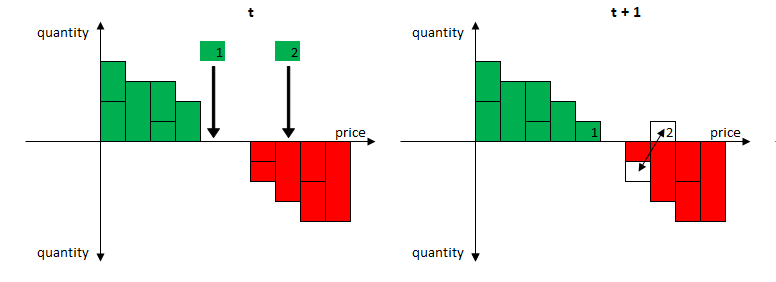
\includegraphics[width=15cm]{diagrams/lob_evolution.png}
        \caption{Evolution of a limit order book}
        \label{fig:lob_evo}
    \end{center}
\end{figure}

% Price formation in continuous settings
Price formation in continuous double auction is rather straight forward. Continuous
market do not allow clearable orders to stay in the limit order book thus the
candidates for trades can be narrowed down only to the opposing orders with better
or equal price than the newly arrived order. This is because the steps for 
clearing is conducted each time a new order arrives.



As ACF and PACF require stationary data, the 
first 100 trading sessions are filtered out in order to start the time series from where
the market has reached the equilibrium.




% Model, stylized facts
In order to increase the robustness of estimating whether the market prices have fat tails or not, the parameters of the
simulations are left unchanged except that the simulation is extended to 10 000 sessions. Jarque-Bera goodness of fit test,
which was used to determine if the distributions are normal or not, require substantial sized sample in order to be accurate.
The null hypothesis of Jarque-Bera test is a joint hypothesis of that the distribution has no skewness and excess kurtosis. 
As can be observed from ~\ref{fig:basic_return_distr_per_session} and ~\ref{fig:basic_return_distr_intrasession}, the last 
prices of sessions are normally distributed but not the intrasession prices. The p-values of Jarque-Bera test suggests similar
results: 0.73 and 0.00 respectively. Therefore the null hypothesis is rejected for the intrasession returns but not for
end of session returns. This is inline with the findings of \citet{Raberto05}. However \author{Raberto05} had slightly
different market structure: their model's order book was emptied after each trading day and ...
\author{Raberto05} did not discuss about the fat tailed returns more than that they are formed due to the market microstructure.
The spike in the distribution of the intrasession returns may be caused by the structure of the order book. If the order book 
sides are steep, as observed in this simulation illustrated in ???, it requires substantially sized order to push the opposing 
side back and have a significant effect on the price. Therefore the price changes between trades are generally rather small
until there comes an order that can buy or sell significant chunk of the opposing side and have instant impact on the price. 
In such a case the opposing side may be weakened so much that the price change can be radical. Therefore the reason for the
spike in the returns may be caused by the occurence that small and medium sized orders may have similar impact on the price
but big orders may push the side relatively much more further as the density of the order quantitity drops when moving further
away from the last market price.


The returns of the market prices after each session are not fat-tailed distributed as can be observed from the figure 
~\ref{fig:basic_return_distr_per_session} but the intrasession . This is somewhat expected: the order prices themselves are drawn from a normal distribution.
However, the returns between trades do diverge from normal distribution, as can be observed ~\ref{fig:basic_return_distr_intrasession} 
from  but this occurs due to the effects the of microstructure in short term. If one order has high quantity and 
relatively attractive price the order might get matched multiple times in a row resulting in the spike of zero return 
shown in the figure. One option to produce the fat-tailed distributions could be to shift the mean of the normal distribution, 
which is used to draw the order prices, depending on whether the order is a bid or an ask. 




One could expect such
a behaviour to be caused by the traders' option of not changing their active order which happened with a probability of
one-third per placement. As the price in each order
is dependent on the market price which existed when the order was created and as there is a chance that
this order will stay in the order book for some time, therefore the market price in the past has influence on the
current structure of the order book as some of the orders are carried to future state of the market. 
In other words, a past market prices may have effect on the upcoming prices via the order book.
This phenomenon can be interpret from the figure ~\ref{fig:basic_market_depth_equilibrium}: the valley
formed by the sides of the order book resembles river.

% The real reason for the autocorrelation
However, this is not the underlying reason for the existence of the autocorrelation. There is similar type and
magnitude of autocorrelation when the option of doing nothing is taken away. This can be observed in the figure 
~\ref{fig:forcesub_autocorr}. This suggests that the autocorrelation is not caused by the order book structure
as in the said experiment the order book reconstructed during each session. Furthermore, as the investors themselves are
not aware of the past and only their positions are the only component reflecting the past, explanation for the 
autocorrelation lies in these positions. Even though the total amount of currency and stock stay constant throughout
trading sessions the distribution of the assets among the traders do not. The relationship between the imbalance
of the assets between the traders, represented as the standard deviation of the positions among the traders, and
the next session's last market price is studied using a multivariate linear regression. This model's performance is
shown in the table ~\ref{tbl:price_explanation}. The model is statistically significant as the p-value of f-statistics
is near zero. In addition, the coefficient of determination, called R squared, is as high as 0.999 meaning that
almost all of the variance in the next session's price is explained by the regression model. To summarize, the
autocorrelation is caused by the imbalance of the positions among the traders and not by the market microstructure
or as a direct result of the decision mechanics of the traders. There is significant multicollinearity in the regression
model thus the individual coefficients or the p-values of the explanatory variables cannot be interpret but this 
does not as is affect to the predictability of the model. 


%\begin{figure}
%    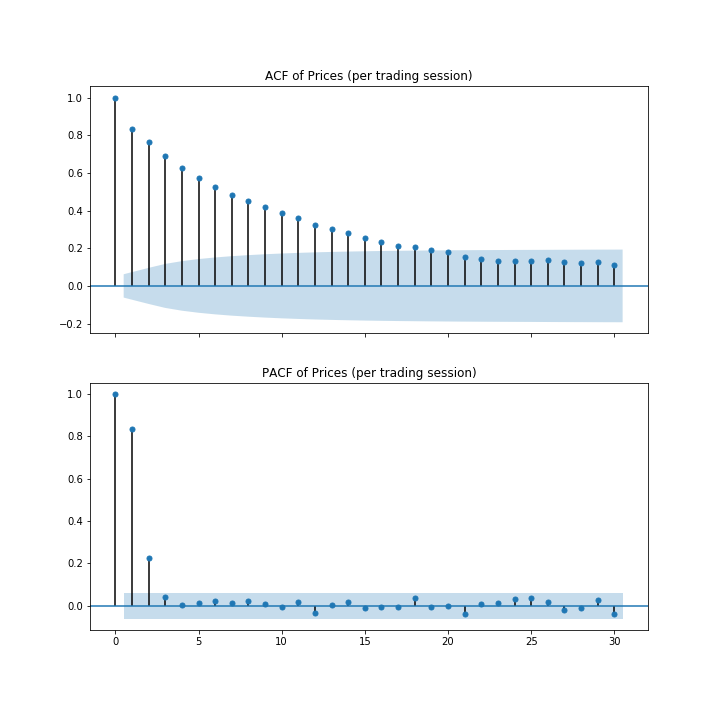
\includegraphics[width=\linewidth]{plots/forcesub_autocorrelation.png}
%    \caption{Autocorrelation of the simulation of no option for inaction}
%    \label{fig:forcesub_autocorr}
%\end{figure}

%\begin{table}
%    \begin{center}
\begin{tabular}{lclc}
\toprule
\textbf{Dep. Variable:}                            & Last price per session, shifted 1 & \textbf{  R-squared (uncentered):}      &     0.999   \\
\textbf{Model:}                                    &                OLS                & \textbf{  Adj. R-squared (uncentered):} &     0.999   \\
\textbf{Method:}                                   &           Least Squares           & \textbf{  F-statistic:       }          & 5.924e+05   \\
\textbf{Date:}                                     &          Mon, 22 Jun 2020         & \textbf{  Prob (F-statistic):}          &     0.00    \\
\textbf{Time:}                                     &              21:47:20             & \textbf{  Log-Likelihood:    }          &   -4731.1   \\
\textbf{No. Observations:}                         &                  999              & \textbf{  AIC:               }          &     9466.   \\
\textbf{Df Residuals:}                             &                  997              & \textbf{  BIC:               }          &     9476.   \\
\textbf{Df Model:}                                 &                    2              & \textbf{                     }          &             \\
\bottomrule
\end{tabular}
\begin{tabular}{lcccccc}
                                                   & \textbf{coef} & \textbf{std err} & \textbf{t} & \textbf{P$> |$t$|$} & \textbf{[0.025} & \textbf{0.975]}  \\
\midrule
\textbf{Std Dev of currency positions per session} &       0.0002  &      3.8e-06     &    50.178  &         0.000        &        0.000    &        0.000     \\
\textbf{Std Dev of stock positions per session}    &      -0.0515  &        0.004     &   -14.215  &         0.000        &       -0.059    &       -0.044     \\
\bottomrule
\end{tabular}
\begin{tabular}{lclc}
\textbf{Omnibus:}       & 13.010 & \textbf{  Durbin-Watson:     } &    0.865  \\
\textbf{Prob(Omnibus):} &  0.001 & \textbf{  Jarque-Bera (JB):  } &   21.220  \\
\textbf{Skew:}          &  0.002 & \textbf{  Prob(JB):          } & 2.47e-05  \\
\textbf{Kurtosis:}      &  3.714 & \textbf{  Cond. No.          } & 2.88e+04  \\
\bottomrule
\end{tabular}
%\caption{OLS Regression Results}
\end{center}

Warnings: \newline
 [1] Standard Errors assume that the covariance matrix of the errors is correctly specified. \newline
 [2] The condition number is large, 2.88e+04. This might indicate that there are \newline
 strong multicollinearity or other numerical problems.% table.tex > \mytable
%    \caption{Linear regression explaining future price with the Standard deviation of stock and currency positions per session}
%    \label{tbl:price_explanation}
%\end{table}

% Proposion to real markets
This finding also has a proposion for real markets: the price may also be driven by the imbalance of wealth between traders 
not just the total amounts of assets. For example, if one buyer has excess cash compared to other investors that buyer is more 
inclined to make a bid order of higher value than others. This buyer has an option to overshoot the price by buying 
significant block of the ask side increasing the market price rapidly but this kind of burst less likely if the cash 
is equally distributed among the buyers and the buyers make decisions independently. In the latter case there is less
impact for each buyer to the market price thus such burst of price would require coordination between the buyers.

% How to fix autocorrelation
To reduce the autocorrelation, one option would be to increase the amount of traders to dilude the effect as then
one trader skewing their positions has little impact on the price dynamics. Another option would be to change the 
distribution or logic how the traders pick amount of currency and stock to allocate to each order.In addition, 
\citet{StylizedFacts01} also discussed that also the real markets may have some autocorrelation 
of returns for small intraday time periods, such as 20 minutes, and therefore one trading session in the simulation 
may be more closer, in terms of comparison, to an intraday time period. However, they stated this autocorrelation
to be caused by market microstructure and as this could be also a cause in the autocorrelation in the simulation,
the more impactful component is the asset imbalance with current simulation parameters and implementation.
